%----------------------------------------------------------------------------------------
%	PACKAGES AND OTHER DOCUMENT CONFIGURATIONS
%----------------------------------------------------------------------------------------

\documentclass[paper=a4, fontsize=11pt]{scrartcl} % A4 paper and 11pt font size

\usepackage[T1]{fontenc} % Use 8-bit encoding that has 256 glyphs
\usepackage{fourier} % Use the Adobe Utopia font for the document - comment this line to return to the LaTeX default
\usepackage[english]{babel} % English language/hyphenation
\usepackage{amsmath,amsfonts,amsthm} % Math packages
\usepackage{lipsum} % Used for inserting dummy 'Lorem ipsum' text into the template

\usepackage{caption}
\usepackage{subcaption}
\usepackage{graphicx}

\usepackage{float}

\usepackage{blindtext} %for enumarations

\usepackage[]{hyperref}  %link collor

%talbe layout to the right
%\usepackage[labelfont=bf]{caption}
%\captionsetup[table]{labelsep=space,justification=raggedright,singlelinecheck=off}
%\captionsetup[figure]{labelsep=quad}

\usepackage{sectsty} % Allows customizing section commands
\allsectionsfont{\centering \normalfont\scshape} % Make all sections centered, the default font and small caps

\usepackage{fancyhdr} % Custom headers and footers
\pagestyle{fancyplain} % Makes all pages in the document conform to the custom headers and footers
\fancyhead{} % No page header - if you want one, create it in the same way as the footers below
\fancyfoot[L]{} % Empty left footer
\fancyfoot[C]{} % Empty center footer
\fancyfoot[R]{\thepage} % Page numbering for right footer
\renewcommand{\headrulewidth}{0pt} % Remove header underlines
\renewcommand{\footrulewidth}{0pt} % Remove footer underlines
\setlength{\headheight}{13.6pt} % Customize the height of the header

\numberwithin{equation}{section} % Number equations within sections (i.e. 1.1, 1.2, 2.1, 2.2 instead of 1, 2, 3, 4)
\numberwithin{figure}{section} % Number figures within sections (i.e. 1.1, 1.2, 2.1, 2.2 instead of 1, 2, 3, 4)
\numberwithin{table}{section} % Number tables within sections (i.e. 1.1, 1.2, 2.1, 2.2 instead of 1, 2, 3, 4)

%\setlength\parindent{0pt} % Removes all indentation from paragraphs - comment this line for an assignment with lots of text


\setlength\parskip{4pt}

%----------------------------------------------------------------------------------------
%	TITLE SECTION
%----------------------------------------------------------------------------------------

\newcommand{\horrule}[1]{\rule{\linewidth}{#1}} % Create horizontal rule command with 1 argument of height

\title{	
\normalfont \normalsize 
\textsc{Ferdowsi University of Mashhad} \\ [25pt] % Your university, school and/or department name(s)
\horrule{0.5pt} \\[0.4cm] % Thin top horizontal rule
\huge  Literature review for Deep Reinforcement Learning Based Mobile Robot Obstacle Avoidance \\ % The assignment title
\horrule{2pt} \\[0.5cm] % Thick bottom horizontal rule
}

\author{Soroush Naseri, Zahra Niazi} % Your name

%\date{\normalsize\today} % Today's date or a custom date

\begin{document}
%\nocite{*}
\maketitle % Print the title

% \newpage
% \begin{abstract}

% {\noindent{\Large Abstract} }\\

% and the method of reduce energy consumption.  \\


% \textbf{Key words:} 
    
% \end{abstract}

\newpage
\tableofcontents

%----------------------------------------------------------------------------------------
%	Section 1
%----------------------------------------------------------------------------------------

%how to cite
%\cite{Seow2011}
%how to add figure



\newpage
\section{Introduction}

\subsection{Obstacle Avoidance using RL and DL}
The navigation capability is a fundamental problem of mobile robots, which include unmanned vehicles, aerial vehicles, and ships. The general aim of navigation is to identify an optimal or sub-optimal path from a starting point to a target point in a Two-Dimensional (2D) or Three-Dimensional (3D) environment while avoiding obstacles. Delivery robots, warehouse automated guided vehicles, and indoor service robots require robust robot navigation systems in their dynamic environments. 
Adding autonomous navigation ability to robot platforms boosts their performance significantly since they can reach wherever they are needed on their own. This motivation has driven researchers to push the autonomous navigation technology to its limits.
Over the years, computers have evolved dramatically reducing the computational burden for mobile robot platforms. This has paved the road toward using more powerful methods like DL and reinforcement learning which have higher processing power requirements.
Inspired by interesting learning results achieved by RL, it has been extended to handle problems with continuous state and action spaces. This trend has been reinforced by borrowing ideas from DL giving birth to robust deep RL (DRL) methods capable of controlling robots with continuous and high dimensional states and action spaces. For example, Cheng et al.\cite{Cheng2022} applied DRL for path following and obstacle avoidance.



\subsection{DRL-based Navigation}

Mobile robots include unmanned vehicles, aerial vehicles, and ships that move in two or three dimensions. Their navigation involves searching for an optimal or sub-optimal path from the starting point to a target point while avoiding obstacles. To simplify this challenge, most researches have focused only on the navigation problem in 2D space.
The purpose of using a DRL algorithm in an autonomous navigation task is to find the optimal policy for guiding the robot to its target position through interaction with the environment. Many well-known DRL algorithms, such as DQN\cite{mnih2013}, DDPG\cite{lilli2015}, PPO\cite{schulman2017}, and their variants, have been extended to realize a DRL-based navigation system. These methods describe the navigation process as an MDP that uses sensor observation as the state with the goal of maximizing the expected revenue of the action. As mentioned above, DRL-based navigation has the advantages of being mapless and having a strong learning ability and low dependence on sensor accuracy. As RL is a trial- and-error learning technology, the physical training process inevitably leads to collisions of the robot with environmental obstacles, which is prohibited. Generally, the deep neural network is trained in a simulation environment before being deployed in a real robot for real-time navigation decision making.
DRL-based navigation has been used to replace or be integrated into the traditional navigation framework. Figure \ref{fig:DRLNavSys} shows the interaction process between the agent and environment of the DRL-based navigation system. The DRL agent replaces the localization and map building module as well as the local path planning module of the traditional navigation framework, moving toward the target point while avoiding static, dynamic, and simple structurally continuous obstacles. However, in an environment where structurally continuous obstacles are too complex, the agent may fall into a local trap. In this case, DRL requires additional global information provided by the traditional navigation technique.
 
\begin{figure}[h!]
	\centering
	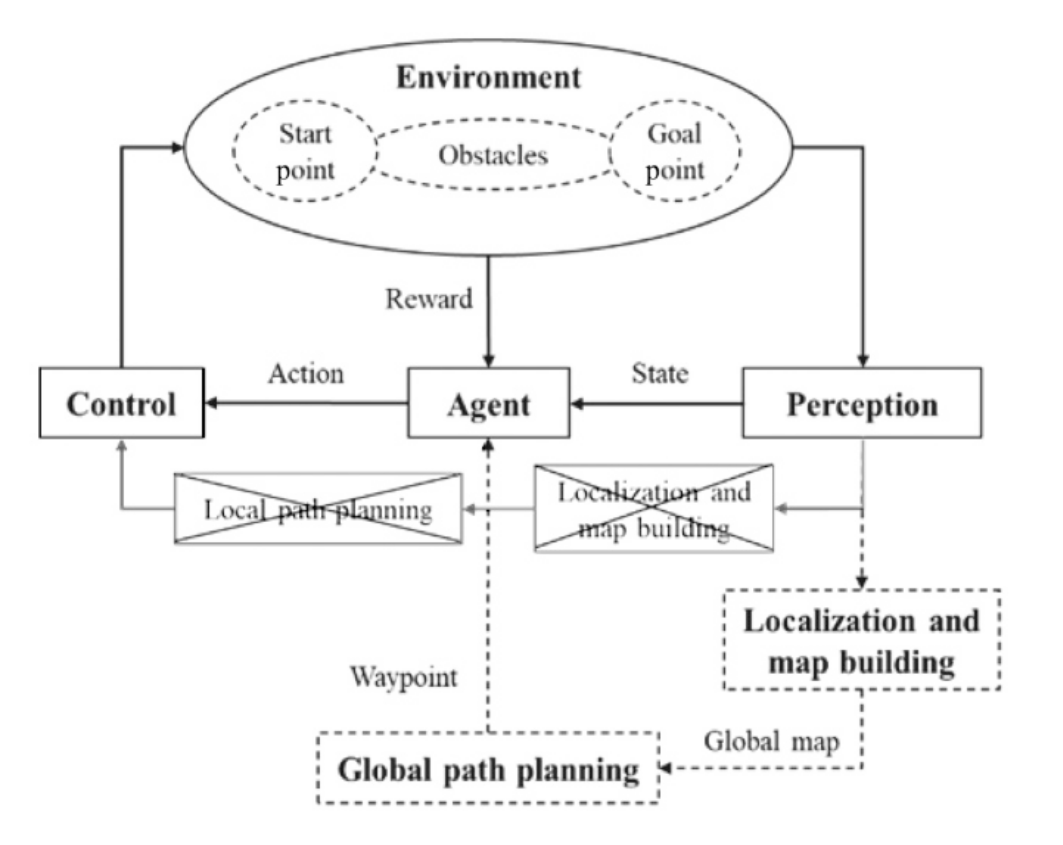
\includegraphics[width=0.8\linewidth]{figures/drl-based-nav.png}
	\caption{DRL-based Navigation System}
	\label{fig:DRLNavSys}
\end{figure}




%----------------------------------------------------------------------------------------
%	Section 2
%----------------------------------------------------------------------------------------

\newpage
\section{Application Scenario}
\label{chapter2}
\textit{}
%---- the scope of this chapter}}

In this review, we divide the application scenarios of DRL navigation into four categories: local obstacle avoidance, indoor navigation, multi-robot navigation, and social navigation. A simple comparison of these scenarios is shown in Table \ref{tb:drlNav}. Each scenario has
the same basic navigation tasks but features different emphases and details. The local obstacle-avoidance scenario emphasizes dynamic changes in the simple structural environment, whereas indoor navigation
focuses on the complexity of the indoor structural environment. The multi-robot navigation scenario involves an environment with multiple high-speed mobile robots. Social navigation focuses on moving through pedestrian-rich environments. In this review our main focus is on local obstacle avoidance and indoor navigation.

\begin{table}[H]
% \centering
\caption{Simple comparison of different DRL-based navigation scenarios.}
\label{table:symbols}
\begin{tabular}{p{2cm}p{1.5cm}p{1.5cm}p{1.5cm}p{1.5cm}p{1.5cm}p{2cm}p{1.5cm}}
\hline
Navigation Scenario & Static obstacle & Dynamic obstacle & Structured continuous obstacle & Obstacle scale & Obstacle velocity & Cooperation & Randomness \\ \hline
Local obstacle avoidance & Y & Y  & N & Low & Low & - & - \\
Indoor navigation & Y & N  & Y & Low & - & - & - \\
Multi-robot navigation & Y & Y  & N & High & High & Y & Low \\
Social navigation & Y & Y  & N & High & High & N & High\\ \hline
\end{tabular}
\label{tb:drlNav}

\end{table}

\begin{figure}[h!]
	\centering
	\includegraphics[width=0.8\linewidth]{figures/Drl-based-navigation.png}
	\caption{Four application scenarios of DRL-based navigation.}
	\label{fig:DRLNavScenario}
\end{figure}


\subsection{Local Obstacle Avoidance}
\subsubsection{Feature}
As mobile robots navigate through their operational environment, they have to deal with variety of obstacles in order to reach their destination. Therefore, the ability to avoid obstacles during navigation is a crucial module in autonomous systems. The location of obstacles may be known as part of the environment map but oftentimes the map is not known beforehand. Thus, it is highly desirable for autonomous mobile robots to be able to detect and avoid obstacles in real- time during navigation. Several obstacle avoidance methods exist in the literature which are reviewed in this section.
The local obstacle-avoidance scenario, which is the most common application scenario of the DRL-based navigation system, is the basis of the other scenarios and can be extended to more complex navigation tasks. In traditional navigation frameworks, reactive methods
are typically used to solve this type of problem, such as the APF or velocity-based methods. One of the biggest problems of reactive methods is the need for a good sensor system that can generate accurate position coordinates for any local obstacle. DRL methods
implicitly process sensor data through neural networks, which overcome the shortcomings of traditional obstacle- avoidance methods. The energy calculation for life cycle inventory is basically similar for all the production processes. 

\subsubsection{Development}
In 2016, Duguleana and Mogan\cite{duguleana2016} studied autonomous navigation in environments containing static and dynamic obstacles; they combined the neural network Pose-Net and a 30-20-3 multi-layer perceptron with the famous RL method Q learning\cite{watkins1989}. By dividing the surrounding obstacle environment into eight angular regions, they reduced the number of states. Pose-Net can output three discrete actions, i.e., moving forward, turning left, and turning right. This early research realized effective obstacle avoidance in simple physical environments. Subsequently, DRL solutions, such as DQN, were rapidly developed, receiving widespread attention. In numerous works, mature DRL methods have been applied to local obstacle-avoidance scenarios. Feng et al.\cite{feng2019} used DDQN to train the agent in a simulation environment to avoid collisions with a wall without using a target point.

\subsubsection{Sensor Robustness}
In most studies, DRL-based navigation applications must be deployed using the same sensors as those used in the training environment. When faced with different hardware conditions, the system may fail. Aznar et al.\cite{aznar2019} designed a navigation policy specifically for fault tolerance, whereby the proposed system can continue to work normally under sensor failure conditions and shows several advantages in its robustness, scalability, and practicality. Choi et al.\cite{choi2019} studied the limited Field Of View (FOV) problem. They transformed depth data obtained by a D435 depth camera with a FOV of 90ı into distance data and proposed a Long Short-Term Memory (LSTM) agent with a Local-Map Critic (LSTM- LMC) that has memory ability. The proposed method improves the robustness of DRL agents in the real world by introducing a dynamics randomization technique, including scan noise, velocity randomization, and time-scale randomization. In addition, the sensors on the robot
can be replaced, or the parameters can be changed (e.g., the resolution and range of the lidar can be changed). Using another approach to solve the sensor robustness problem, Leiva and Ruiz-del-Solar\cite{leiva2020} incorporated the corresponding angle of the range measurement as part of the observation, which allows the learning of features that are independent of the geometric distribution of the readings. The authors used variably sized 2D point clouds as the agent’s 2D observations, thereby improving robustness and extensibility to the real world.


\subsection{Indoor navigation}
\subsubsection{Feature}
Here, the indoor navigation scenario refers to a house with multiple rooms or a 3D maze-like environment with numerous walls and corridors. Although the local obstacle-avoidance scenarios in the previous section may also be indoors, their structures are often relatively simple. In this section, we focus on indoor navigation scenarios with a complex structural environment. 
The A3C algorithm proposed by Mnih et al.\cite{mnih2016} is a representative Actor-Critic (AC) method. The classic policy gradient algorithm directly optimizes the agent’s policy; it must collect a series of complete sequence data to update the policy. In DRL, collecting sequence data is often challenging and large variances can be introduced. The AC structure that combines the value function with the policy gradient method is receiving much attention.
In 2017, Mirowski et al.\cite{mirowski2016} adjusted the network structure of A3C and proposed the Nav A3C algorithm, in which two LSTM layers are added between the CNN and the output layer. However, NAV A3C was found to have an unstable policy, poor data efficiency, and poor robustness in a complex environment. Zeng and Wang\cite{zeng2020} used the monotonic policy improvement advantage of PPO and proposed the appoNav (asynchronous PPO) algorithm to solve the visual navigation problem.
In previous research\cite{zhu2017}, the DRL algorithm was found to be generalizable to new scenarios, but at the expense of a decrease in performance and the need to fine-tune the network. To improve the generalization ability of the visual navigation algorithm, Devo et al.\cite{devo2020} proposed the importance weighted actor–learner architecture, a new framework comprising object localization and navigation networks.





\newpage
\section{Conclusion}
\label{chapter3}


Here we present our problem and the way to tackle it; Consider a maze with flat ground. We place the robot at the start point and we also consider a goal which is located in our maze.
Eddie has to reach the goal and it must use an optimal path to do so. The point is that our maze has lots of obstacles and one of the topics we wish to discuss is static obstacle avoidance.
The method that helps us here is Reinforcement Learning. As previously mentioned, we prefer to use Policy Gradint methods especially A2C. Firstly we define a reward function. Then we define two terms in order to show the angle and the distance of Eddie to the goal and we also consider two -x and +x rewards for collision and reaching the goal respectively. Next we have to construct our actor policy network in order to get the depth image as input and output velocity as an action. We also define a critic network because we have to modify our actor Policy network. To do this we use "Baseline3" library that provides Deep RL algorithms.


%bibliography
\bibliographystyle{abbrv}
\bibliography{sample.bib}

\end{document}